\label{ch:experimental_measurements}
\section{Research Objectives}
After the description of the experimental apparatuses that we used, and a basic explanation of the main principles in glass polishing, we can present the main ideas and goals of the project.
\\
Due to the grinding and polishing process in optics manufacturing, contaminants can leak into the surface of the glass from both the water and the polishing suspension, possibly causing issues in the optical property of the final product.
\\
Our primary research objectives were:
\begin{enumerate}
    \item To confirm the presence of contaminants and to definitively confirm whether contamination actually occurs.
    \item To quantify the magnitude of this effect by measuring the concentration of contaminants at the surface.
    \item To investigate whether the process parameters, like polishing time or polish concentration, can have an influence on the result.
\end{enumerate}
A crucial part of our experience was to investigate whether all these evaluations could be done using a LIBS apparatus.

\section{Polishing Parameters}
\label{sec:pol_parameter}
After having thought about the parameters we could vary, we settled on a collection of variables that we identified as the most relevant:
\begin{itemize}
    \item Polishing time: by increasing the contact time we expect to see changes in the amount of concentration found at the surface.
    \item Polishing agent: expecting that the physical and chemical properties of different agents could have a different interaction with the glass. The two main polishing agents used in optics manufacturing are aluminum oxide (\ce{Al2O3}) and cerium oxide (\ce{CeO2}). The latter also usually contains traces of other elements like carbon or lanthanum.
    \item Type of water: tap water could impact the process by introducing new contaminants. Also, tap and distilled water can differ for chemical properties too, the pH of tap water is usually around 7.4 and distilled water is slightly more acidic with a pH of 5.7, due to the presence of a small amount of carbon dioxide that gets instantly dissolved into the water from the atmosphere [ph water paper].
    \item •	Polish concentration: the common concentrations used in optic manufacturing are between 5\% to 30\% in mass, where the percentage indicates the fraction of the mass of the polishing agent relative to the total weight of the slurry. Concentration influences both the mechanical properties of the solution, by physically having more particles interacting with the surface, and the chemical ones, by changing the alkalinity.
    \item Type of glass: glasses with different compositions are used in optics because their refractive index is strongly dependent on the density of the material and by introducing different and heavier elements in the glass, the manufacturer can tune its optical properties to the desired ones. Having a high concentration of different elemental species inside the glass could change the parameters that regulate diffusion at the surface.
\end{itemize}

\section{Theoretical Prediction}
\label{sec:theoretical_prediction}
As already mentioned in Chapter~\ref{sec:grinding_glass}, the description of the chemical-mechanical polishing is extremely complex, and it would be difficult to develop a model to predict and fit the results to the LIBS measurement.
\\
The simplest approach to describe the presence of contaminants in the glass is diffusion. Specifically, “normal” diffusion, where the concentration follows the two Fick’s laws. In particular, the second Fick’s law states:
\begin{align}
    C\left(x,t\right)=C_0\operatorname{erfc}\left(\frac{x}{2\sqrt{Dt}}\right) \label{eq:second_fick}
\end{align}
In the case of our LIBS measurements, we are not measuring depth resolved data. The laser ablates all the material in a small portion of the surface, and we measure the concentration of all the species that are present from the surface level to the deepest part of the ablated region. We are therefore measuring a quantity that is proportional to the integral of the concentration.
\\
Is it possible to obtain the analytical solution of the integral of the error function, by looking at some tables we find that:
\begin{align}
    \int\operatorname{erfc}\left(az\right)dz=z\operatorname{erfc}\left(az\right)-\frac{1}{a\sqrt\pi}\exp{\left(-a^2z^2\right)} \label{eq:integral_erfc}
\end{align}
In our case the parameter $a$ is equal to $\frac{1}{2\sqrt{Dt}}$. The integral is then evaluated over an interval that starts at 0, that we take as the surface level, and ends at a distance $d_a$, which is the maximum depth of the ablation. It also makes sense to normalize the expression relative to the length by dividing the integral by $d_a$.
\\
The final expression is therefore: 
 \begin{align}
    \overline{C}\left(d_{a},t\right)=C_{0}\int_{0}^{d_{a}}\operatorname{erfc}\left(\frac{x}{2\sqrt{Dt}}\right)\operatorname{d}x=C_{0}\left[d_{a}\operatorname{erfc}\left(\frac{d_{a}}{2\sqrt{Dt}}\right)-2\sqrt{\frac{Dt}{\pi}}\left[\exp\left(-\frac{d_{a}^{2}}{4Dt}\right)-1\right]\right]\frac{1}{d_a} \label{eq:c_bar_equation}
 \end{align}
There are two functional contributions to the expression:
\begin{align}
    g(t) &= d_{a\ }\operatorname{erfc}\left(\frac{d_a}{2\sqrt{Dt}}\right) \label{eq:g_t} \\
    \\[1pt]
    h(t) &= 2\sqrt{\frac{Dt}{\pi}}\left[\exp{\left(-\frac{d_a^2}{4Dt}\right)}-1\right] \label{eq:h_t}
\end{align}
In this way $\overline{C}$ can be written as $\overline{C} = g(t) + h(t)$
\\
By plotting the two contributions and the total function in a logarithmic plot, we can see that $g(t)$ and $h(t)$ intersect.
\\
The time value at the intersection point, $t_s$, separates the domain in two regions:
\begin{figure}[H]
   \centering
   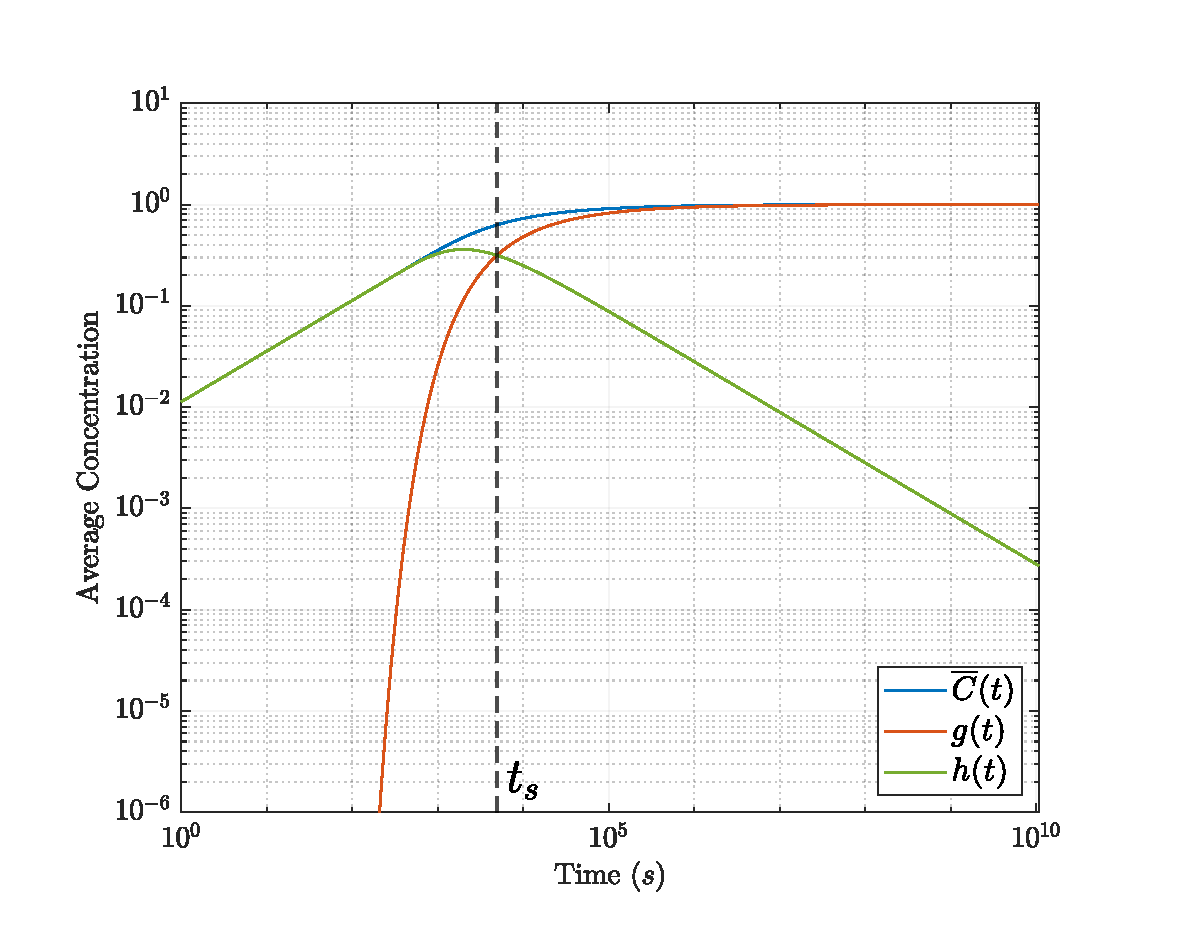
\includegraphics[width = \textwidth]{chapter_3/theoretical_cons/conc3Functions.pdf} 
   \caption{The average concentration and the two functional components. }
   \label{fig:c_bar_plot}
\end{figure}
For $t<t_s$, $h(t)$ is the dominant contribution, and the overall function behaves linearly.
\\
For $t>t_s$, $g(t)$ becomes the dominant contribution. Since $g(t)$ tends to $C_0$, $\overline{C}$ will also tend to the same parameter. Physically, this behavior represents the time values for which the saturation condition, with a homogeneous concentration equal to $C_0$, has been reached in the spatial region between 0 and $d_a$. 
\\
Considering that $D$ is always multiplying $t$, a change in the value of the diffusion coefficient, translates in a rigid shift to the left, by a value equal to $\log_{10}(D)$, of the whole function.
\\
Therefore, looking at a fixed interval of time between $t_1$ and $t_2$, two cases can be distinguished:
\\
If $t_s >> t_2$, corresponding to small values of $D$, the behavior is linear inside the considered region, and saturation is not reached.
\begin{figure}[H]
   \centering
   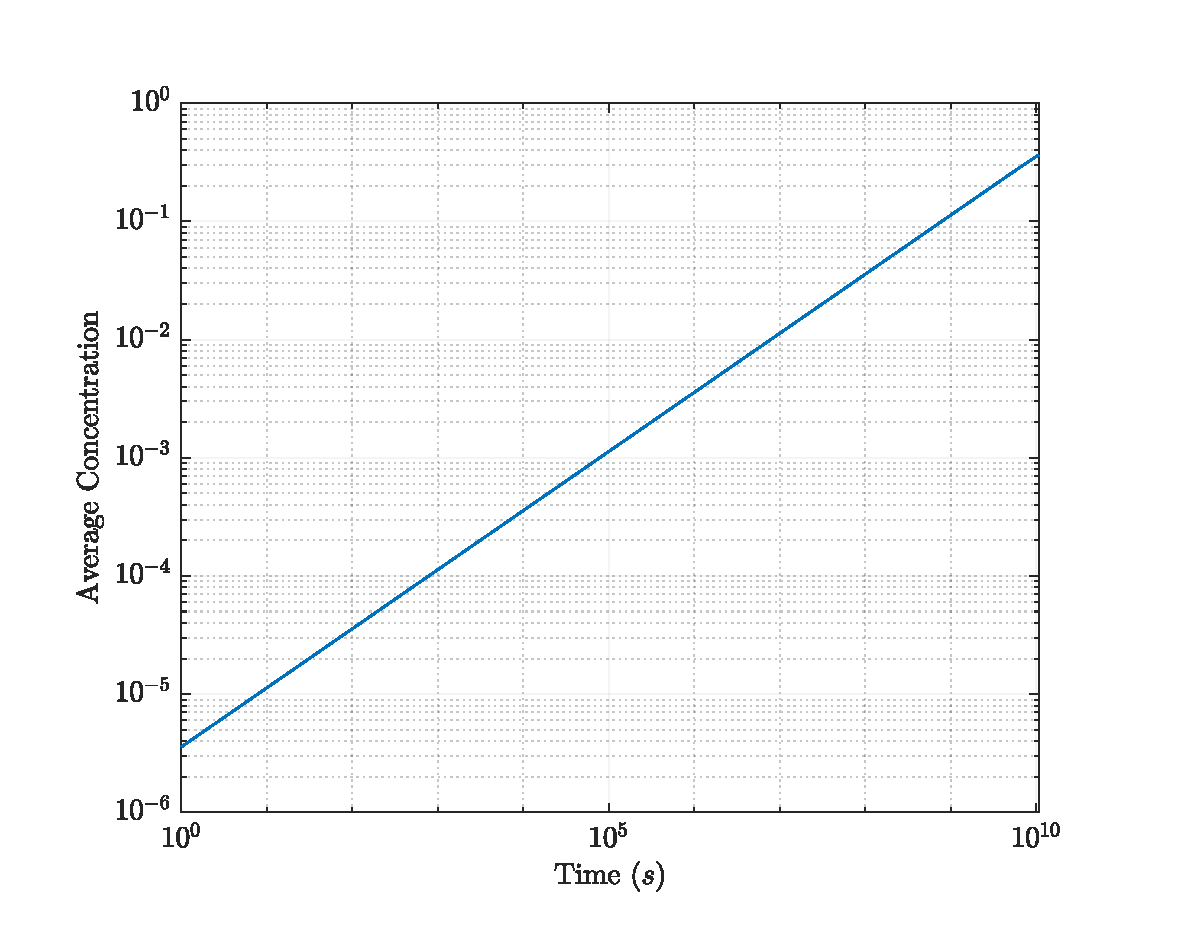
\includegraphics[width = \textwidth]{chapter_3/theoretical_cons/concRegim_linear.pdf} 
    \vspace*{-30pt}
   \caption{Linear behavior of $\bar{C}$ for $\protect t_s >> t_2$.}
   \label{fig:c_bar_linear}
\end{figure}
If $t_s ~ t_1$, corresponding to the case of a high value of $D$, saturation is reached almost instantly, and the behavior cannot be considered linear anymore.
\begin{figure}[H]
   \centering
   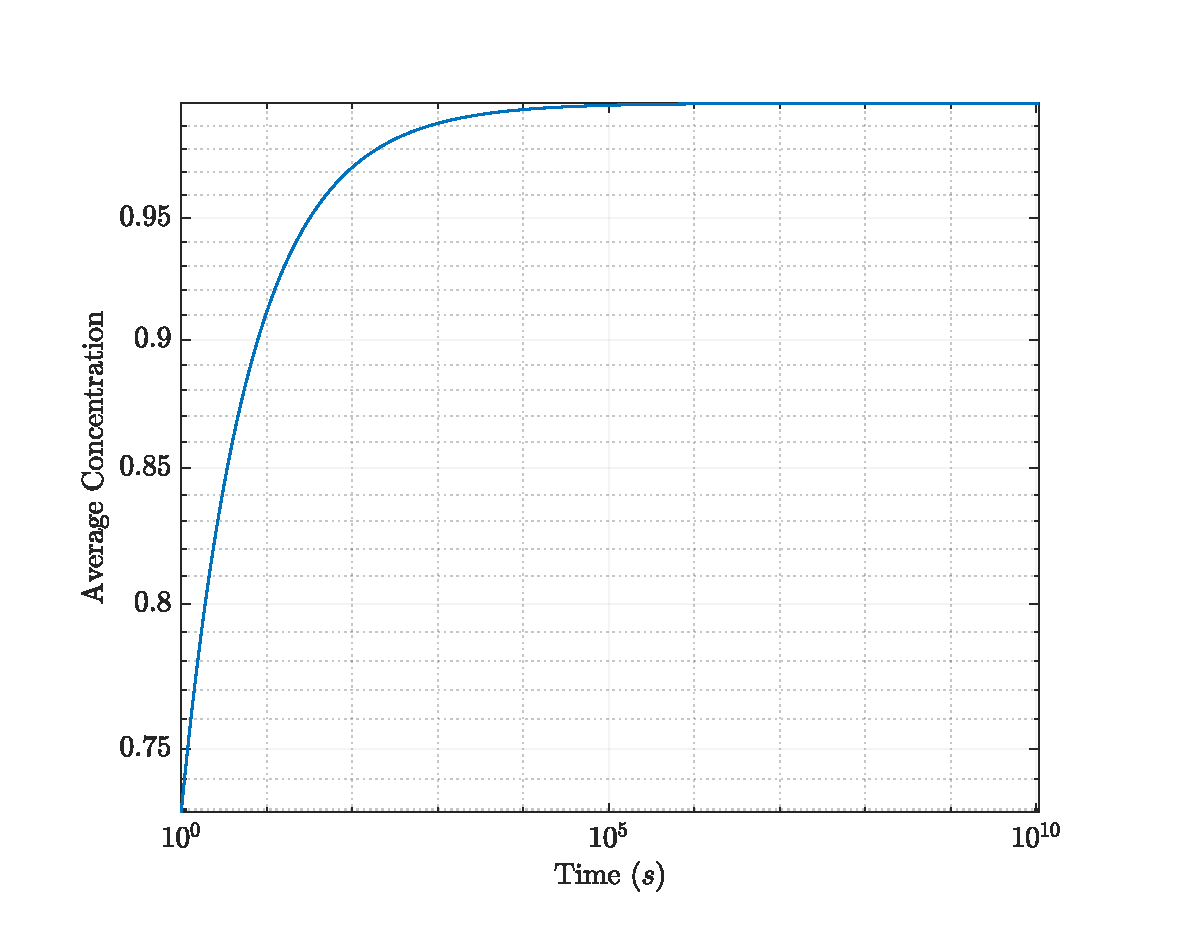
\includegraphics[width = \textwidth]{chapter_3/theoretical_cons/concRegim_exp.pdf} 
    \vspace*{-30pt}
   \caption{Non-linear behavior of $\bar{C}$ for $\protect t_s ~ t_1$.}
   \label{fig:c_bar_non_linear}
\end{figure}
If $t_s \in [t_1, t_2]$, both behaviors are present, and saturation is reached after a period of linear regime.
\begin{figure}[H]
    \centering
    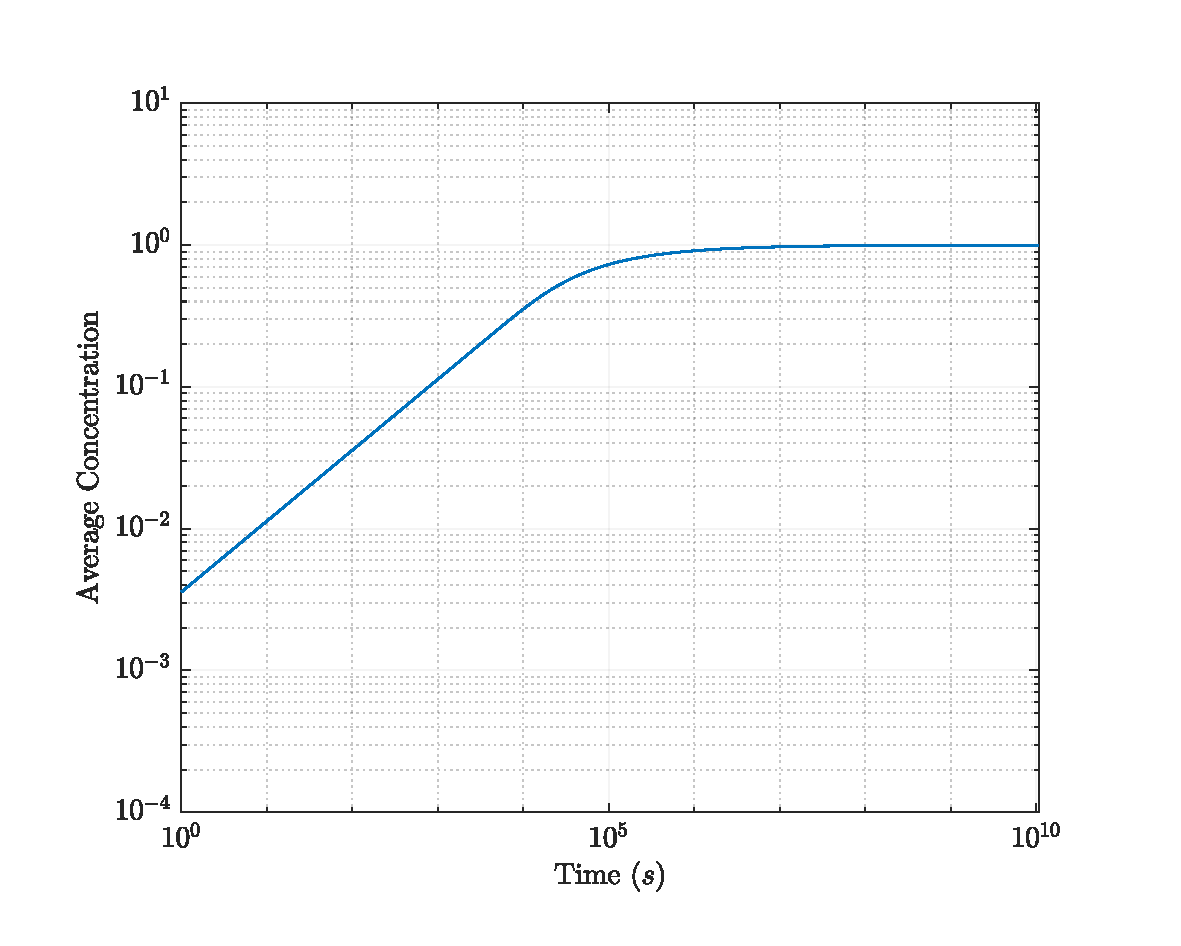
\includegraphics[width = \textwidth]{chapter_3/theoretical_cons/concRegim_mixed.pdf} 
     \vspace*{-30pt}
    \caption{General behavior of $\bar{C}$ for  $t_s \in [t_1, t_2]$.}
    \label{fig:c_bar_mixed}
 \end{figure}
This discussion is relevant because, if the predominant physical mechanism causing the presence of contaminants in the glass is actually diffusion, we should be able to estimate the value of the diffusion constant by comparing $\bar{C}$ to the data found with LIBS measurements.

\section{LIBS}
\label{sec:Description of the apparatus}
As already anticipated in Chapter~\ref{sec:LIBS}, LIBS setup components are multiple.
\\
This analysis technique needs active elements capable of providing the optical energy needed for plasma formation, and a collection of optical and electronic elements capable of collecting and analyzing emitted light from the plasma.
\\
Due to the large field of application of this technique [Source of the different applications], LIBS setups are expected to vary both in size (static vs portable) and complexity.
\\
Generally, LIBS setups all share the same main elements that are listed below:
\begin{enumerate}
    \item The laser source.
    \item The optical system that focuses the laser light on the sample surface.
    \item A target holder.
    \item The light collection system, needed to convey the generated radiation to the detector.
    \item The detection system, capable of spectrally dispersing the collected light and measuring it using a digital sensor.
    \item A computer to control each previously cited element and to create the final spectrum.
\end{enumerate}
The LIBS measurements presented in this thesis have all been carried out using the same apparatus, a custom-made version of the CORALIS system by Lasertechnik Berlin with the following characteristics.

\subsection{Laser Source}
\label{subsec:laster_source}
A solid state, Nd:YAG laser source has been employed in this setup. The system gave us the possibility of tuning the laser pulse energy from less than $1 \: mJ$,  to more than 100.
\\
The Nd:YAG laser was operated at its fundamental wavelength of $1064 \: nm$ and in the Q-Switching regime, in order to achieve the high enough pulse power capable of igniting the plasma. This pulsed laser regime gives a typical duration of each pulse in the order of $5-10\: ns$ [Handbook of LIBS (other sources are possible)] and in the case of the CORALIS system the machine can provide up to 20 pulses per second, with a repetition rate of 20 Hz.

\subsection{Spectrometer}
\label{subsec:spectrometer}
The choice of the spectrometer is also dependent on the type of application and can range from the use of very simple and inexpensive components, such as line filters capable of monitoring a single predetermined wavelength, to sophisticated spectrographs allowing for the simultaneous analysis of a large spectral region.
\\
The commercially available CORALIS has only one echelle spectrometer that operates in the near-UV range (from 190 to $430 \: nm$) and has a spectral resolution that spans from 13 to $35 \: pm$, with a sensitivity of [].
\\
The modified model that we employed has an additional spectrometer that operates in the visible range (from 405 to $802\: nm$) with a spectral resolution of around $4 \: pm$, with a sensitivity of [].
[we are not sure on the value of the resolution of the Visible spectrometer, and we do not have yet the values for the sensitivity]
\\
The overall spectral region that we could analyze was therefore from 200 to $800 \: nm$.

\section{Parameters Chosen}
\label{sec:parameters_chosen}
The choice of the LIBS parameters is a very crucial step in the analysis process since the quality of the results obtained from the measurements is strongly dependent on their values. In general, there are no parameters that are universally optimal, and their value changes based on the type of material, the geometry of the surface, and the element species that are being investigated.
\\
In order to arrive at the final values we employed, a thorough experimental process has been carried out.
\\
The parameters on which we had full choice were the sequent:
\begin{enumerate}
    \item Laser pulse energy.
    \item Gate width.
    \item Delay time.
    \item Detector gain.
    \item Spatial distribution of the measured points on the sample surface.
    \item Number of points per measurement.
    \item Number of laser pulses per measurement.
    \item Number of cleaning pulses before the measurement.
\end{enumerate}
The choice process for the parameters started by analyzing an NZK-7 glass sample from Schott [need the citation]. The glass sample did not undergo any post-processing phase, like grinding or polishing. From now on we will refer to this type of sample as “RAW”.
\\
The first parameter on which we focused our attention was the laser pulse energy. 
\subsection{Pulse Energy}
\label{subsec:pulse_energy}
Silica glass absorbs radiation very inefficiently in the frequency range of the laser of the apparatus we used, as it is clear from Figure~\ref{fig:glass_transmittance} at $1064 \: nm$ the glass transmittance is basically 100\%. 
\begin{figure}[H]
    \centering
    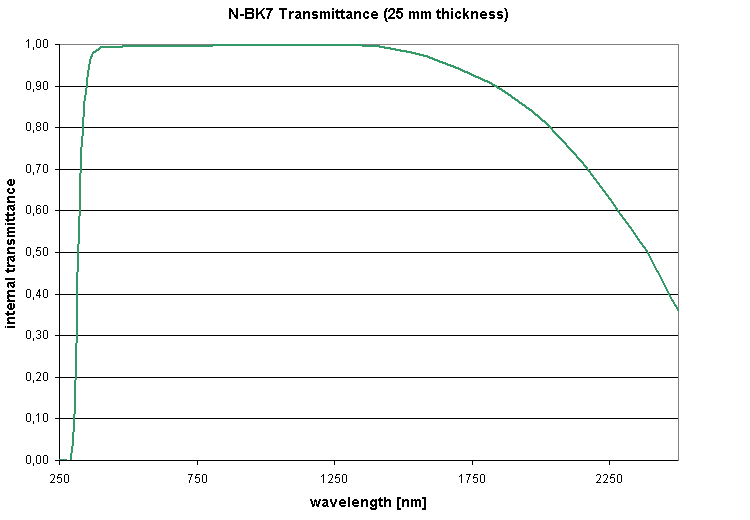
\includegraphics[width = 0.7\textwidth]{chapter_3/tests_graphs/glass_transmittance.png} 
    \caption{Transmittance of N-BK7 glass.}
    \label{fig:glass_transmittance}
 \end{figure}
 Also, in general, the lack of surface features due to polishing and grinding reduces even more the possibility of absorption. To achieve the conditions for breakdown at the surface, a high laser pulse energy must be utilized.
 \\
Tests were carried out from a lower value of $6 \:mJ$ to a higher value of $15\: mJ$.
\\
In Figure~\ref{fig:test_NZK7_6mj} and Figure~\ref{fig:test_NZK7_6mj_zoom} we can see that we already have a good spectrum even with just $6 mJ$.
\begin{figure}[H]
    \centering
    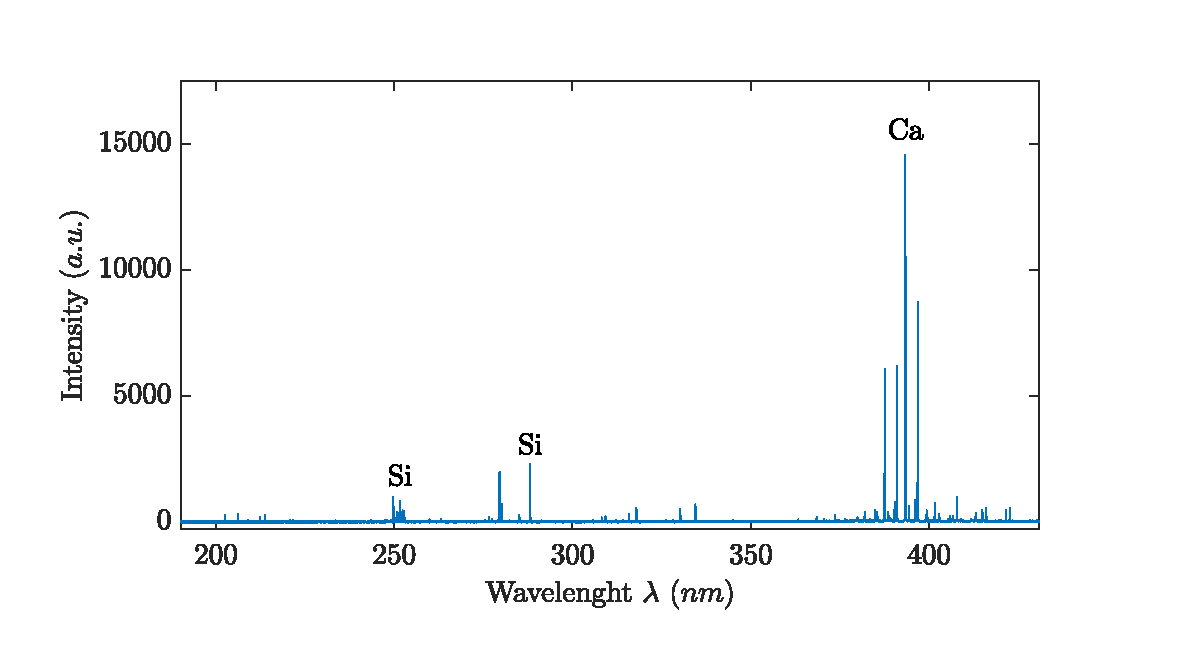
\includegraphics[width = \textwidth]{chapter_3/tests_graphs/test_NZK7_6mj.pdf} 
     \vspace*{-30pt}
    \caption{$\protect 6 \: mJ$ - Spectrum of NZK-7 glass.}
    \label{fig:test_NZK7_6mj}
\end{figure}
\begin{figure}[H]
    \centering
    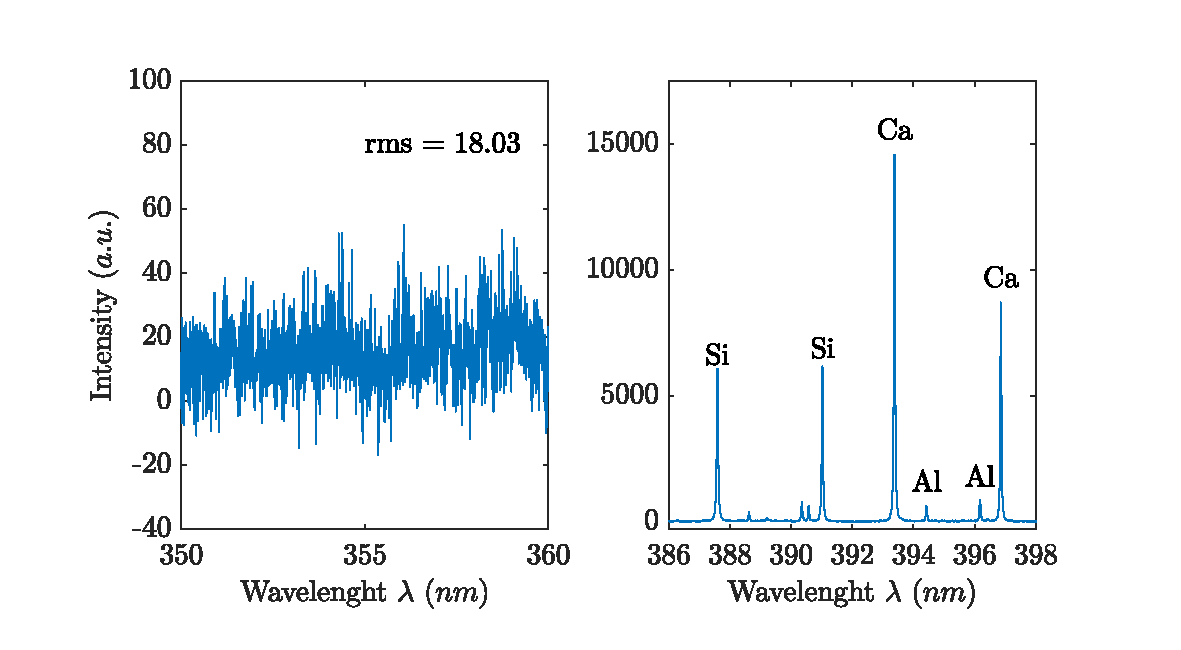
\includegraphics[width = \textwidth]{chapter_3/tests_graphs/test_NZK7_6mj_zoom.pdf} 
     \vspace*{-30pt}
    \caption{$\protect 6 \: mJ$ - (Left) Focus of on the noise. (Right) Focus on the $386 \: nm$ to $398 \: nm$ range.}
    \label{fig:test_NZK7_6mj_zoom}
 \end{figure}
Focusing on the part of the UV spectral range from $386 \: nm$ to $398 \: nm$, we see that the signal-to-noise ratio ($S.N.R$) is about 340 (the value is obtained by dividing the counts of the silicon I peak at $390.55 \: nm$ by the RMS of the noise calculated from $350 \: nm$ to $360 \: nm$).
\\
By increasing the energy value to $10 \: mJ$ we get:
\begin{figure}[H]
    \centering
    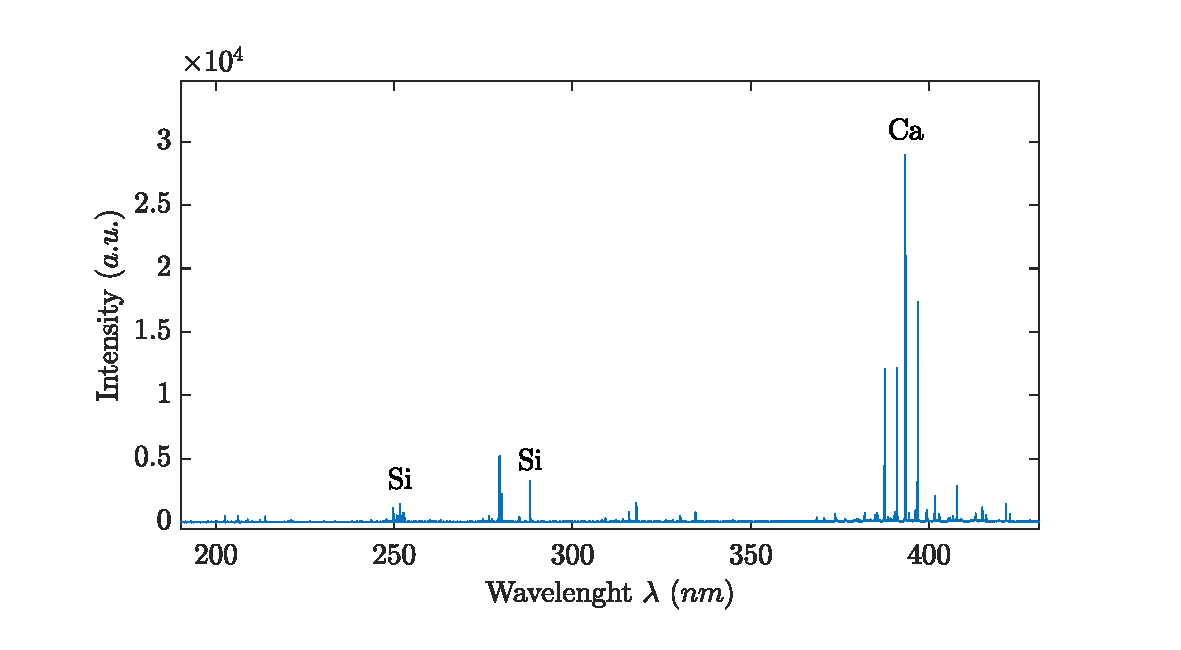
\includegraphics[width = \textwidth]{chapter_3/tests_graphs/test_NZK7_10mj.pdf} 
     \vspace*{-30pt}
    \caption{$\protect 10 \: mJ$ - Spectrum of NZK-7 glass.}
    \label{fig:test_NZK7_10mj}
\end{figure}
\begin{figure}[H]
    \centering
    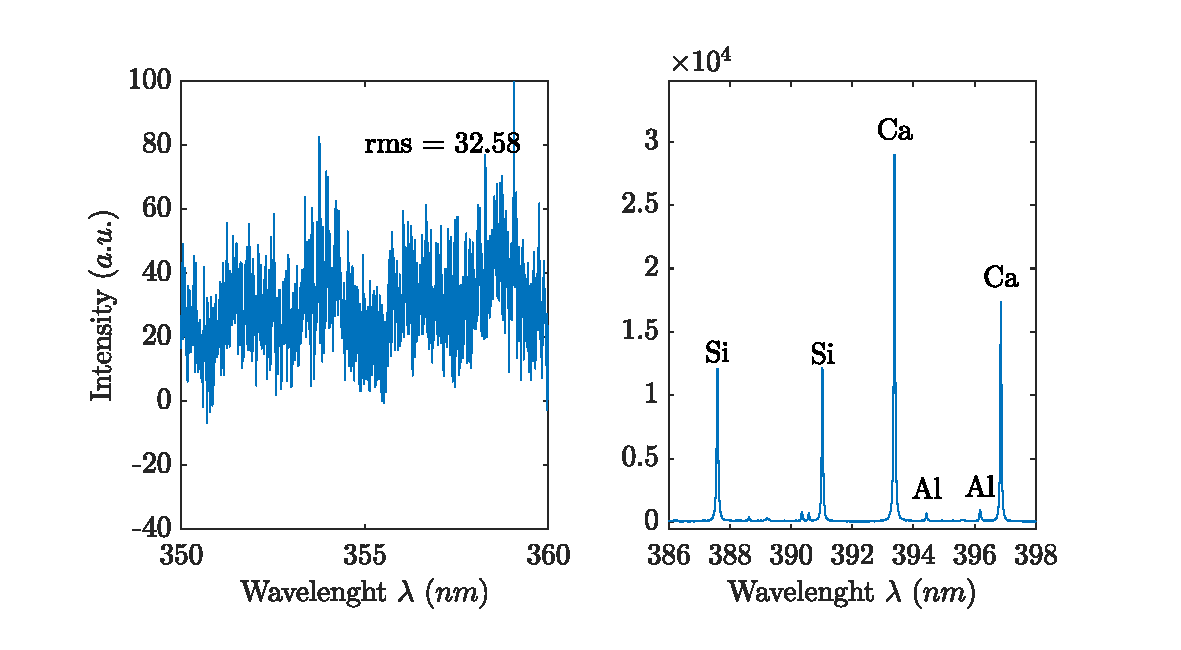
\includegraphics[width = \textwidth]{chapter_3/tests_graphs/test_NZK7_10mj_zoom.pdf} 
     \vspace*{-30pt}
    \caption{$\protect 10 \: mJ$ - (Left) Focus of on the noise. (Right) Focus on the $386 \: nm$ to $398 \: nm$ range.}
    \label{fig:test_NZK7_10mj_zoom}
 \end{figure}
Both the counts and the noise increased with the energy, but the overall $S.N.R.$ is higher, being around 370.
\\
Lastly, we tried $15 \: mJ$:
\begin{figure}[H]
    \centering
    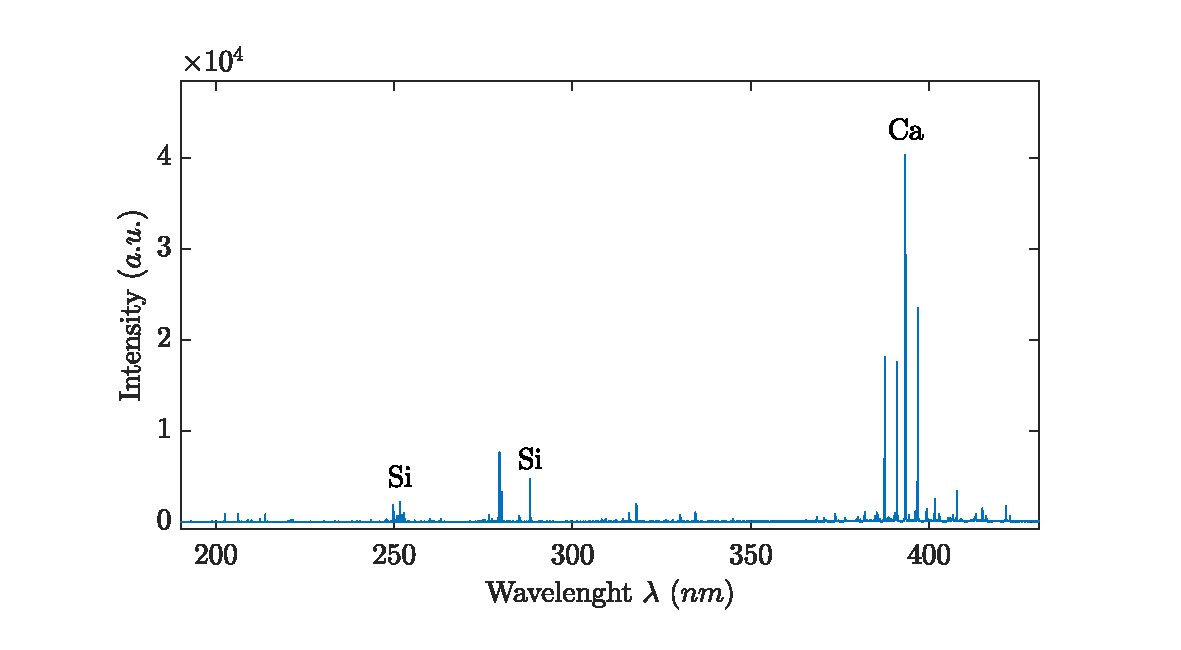
\includegraphics[width = \textwidth]{chapter_3/tests_graphs/test_NZK7_15mj.pdf} 
     \vspace*{-30pt}
    \caption{$\protect 15 \: mJ$ - Spectrum of NZK-7 glass.}
    \label{fig:test_NZK7_15mj}
\end{figure}
\begin{figure}[H]
    \centering
    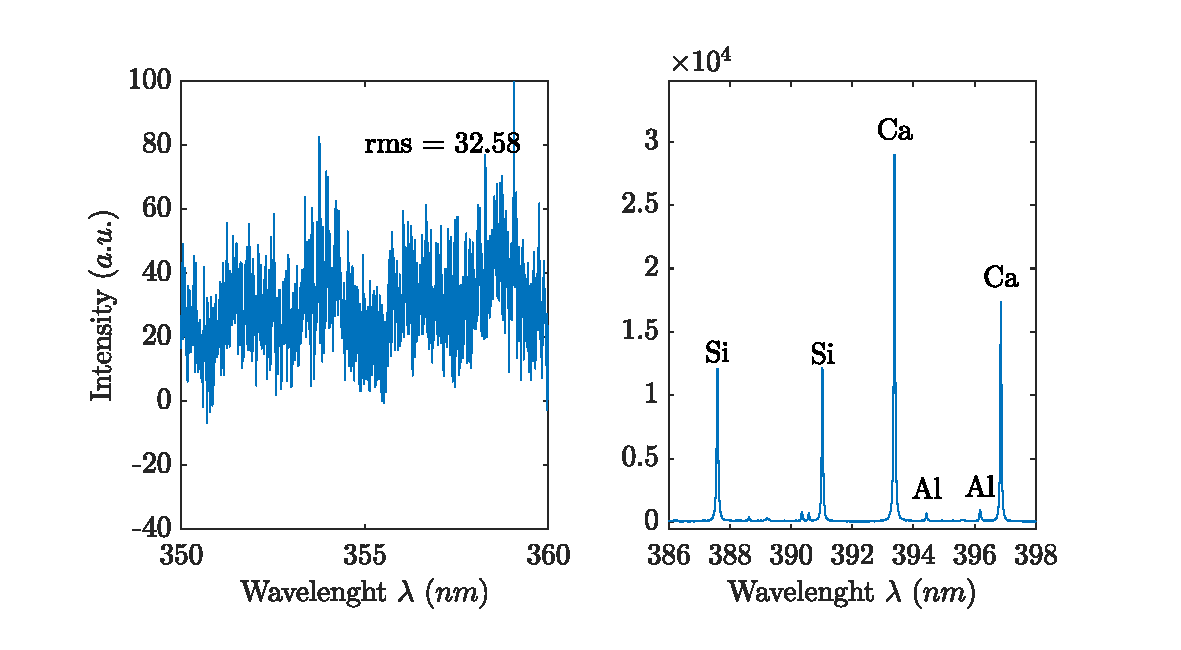
\includegraphics[width = \textwidth]{chapter_3/tests_graphs/test_NZK7_10mj_zoom.pdf} 
     \vspace*{-30pt}
    \caption{$\protect 15 \: mJ$ - (Left) Focus of on the noise. (Right) Focus on the $386 \: nm$ to $398 \: nm$ range.}
    \label{fig:test_NZK7_15mj_zoom}
 \end{figure}

For this value of the energy the $S.N.R.$ is still around 370, so we decided not to increase the energy anymore.
\\
In the end, therefore, we selected $15 \: mJ$ as the final value with which all the measurements have been carried out. 

\subsection{Gate Width and Time Delay}
\label{subsec:gate_width_delay}

To get the values that will give us the most comprehensive plasma spectrum, we decided to perform an analysis called “time evolution”, where the emission spectrum is recorded at various instants in the lifetime of the plasma. To ensure that the plasma parameters, such as electron density ($N_e$) and temperature ($T$), do not vary much within the measurements, in time evolution experiments, the gate width is always set to be equal to half the value of the time delay [jorg’s paper].
\\
The evolution was considered starting from a delay time of $0.5\: \mu s$, that corresponds to a gate width of $0.25 \: \mu s$, to a delay of $10 \: \mu s$ and $5 \: \mu s$ for the gate width.
\\
In Figure~\ref{fig:test_NZK7_time_evo_zoom} we have plotted the intensities of two silicon peaks in two different part of the spectral region for every spectrum of the time evolution. This was done to ensure that the differences measured were homogeneous along the whole frequency range.
\begin{figure}[H]
    \centering
    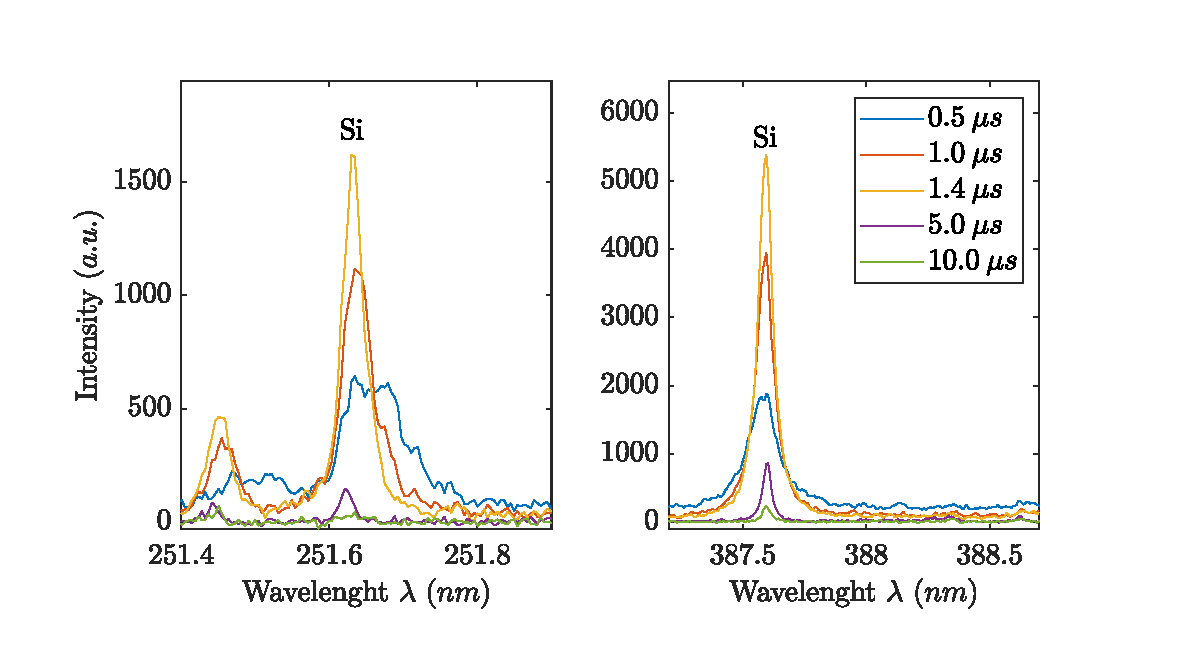
\includegraphics[width = \textwidth]{chapter_3/tests_graphs/test_NZK7_time_evo_zoom.pdf} 
    \vspace*{-30pt}
    \caption[Time evolution.]{Time evolution from $\protect 0.5\: \mu s$ to $10 \: \mu s$. (Left) Silicon peak at $251.63 \: nm$. (Right) Silicon peak at $387.53 \: nm$.}
    \label{fig:test_NZK7_time_evo_zoom}
 \end{figure}

 \begin{figure}[H]
    \centering
    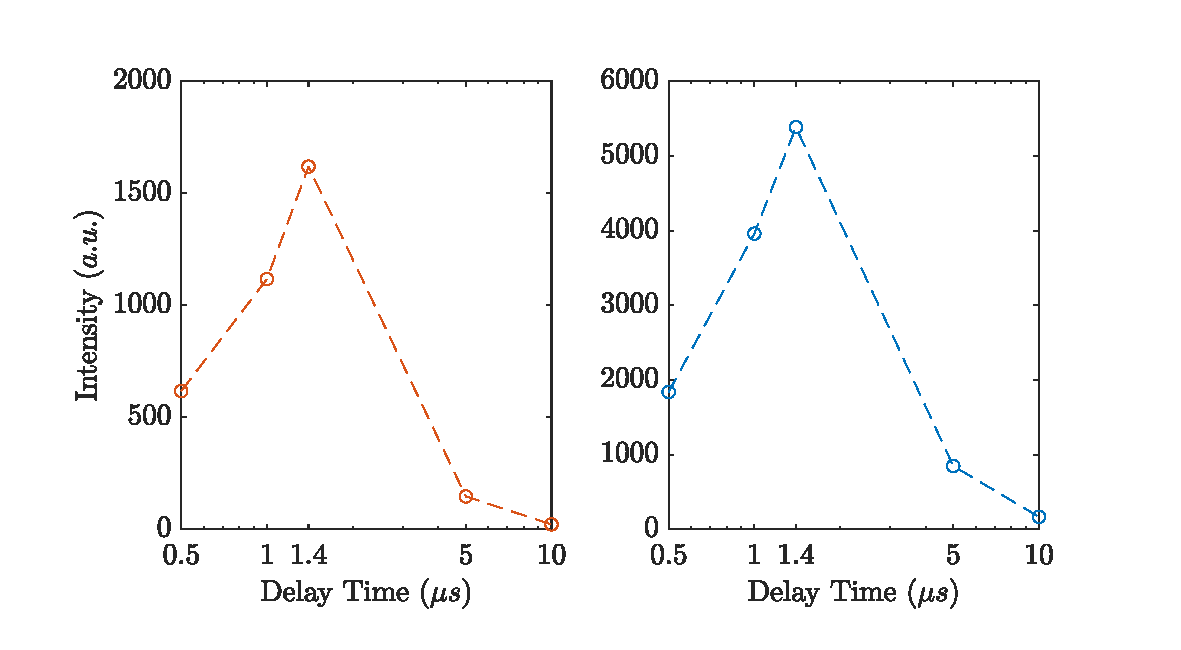
\includegraphics[width = \textwidth]{chapter_3/tests_graphs/time_evo_NZK7.pdf} 
    \vspace*{-30pt}
    \caption{Maximum intensity of the two peaks as a function of the delay time.}
    \label{fig:time_evo_NZK7}
 \end{figure}
In Figure~\ref{fig:time_evo_NZK7} is explicitly shown the maximum intensity of the two peaks as a function of the delay time. The highest intensity corresponds to a time of $1.4 \: \mu s$, and therefore this is the value that we have chosen for our measurements.
\\
Considering that the goal of our research involved finding contaminants that could be in low concentrations, for the gate width we chose a value of $12 \: \mu s$ to collect the highest amount of information possible from the measurements.

\subsection{Detector Gain}
\label{subsec:detector_gain}
The gain of the detector has been set to a value of 3000 because it is the default gain suggested by the manufacturer of the apparatus, and it is usually left unchanged.

\subsection{Number of Points per Measurement}
\label{subsec:number_points_mesurement}